\documentclass[UTF8,fontset=fandol,11pt]{ctexart}
\usepackage[a4paper,margin=24mm,headheight=15pt]{geometry}
\usepackage{amsmath,amssymb,amsthm,mathtools,bm}
\usepackage{enumitem,booktabs,longtable,array,pdfpages,fancyhdr,xcolor}
\usepackage[colorlinks=true,linkcolor=blue!45!black,urlcolor=blue!45!black]{hyperref}
\allowdisplaybreaks[2]
\setlength{\parindent}{2em}
\setlength{\parskip}{3pt}
\setlength{\emergencystretch}{3em}
\setlist{nosep,topsep=3pt}
\pagestyle{fancy}\fancyhf{}\fancyhead[L]{\small 分析学讲义习题解答}\fancyhead[R]{\small 第38--57讲}\fancyfoot[C]{\thepage}
\newcommand{\R}{\mathbb R}\newcommand{\C}{\mathbb C}\newcommand{\N}{\mathbb N}\newcommand{\Z}{\mathbb Z}\newcommand{\Q}{\mathbb Q}\newcommand{\T}{\mathbb T}
\newcommand{\dd}{\,\mathrm d}\newcommand{\eps}{\varepsilon}\newcommand{\ind}{\mathbf1}
\newcommand{\norm}[1]{\left\lVert#1\right\rVert}\newcommand{\abs}[1]{\left|#1\right|}\newcommand{\ip}[2]{\left\langle#1,#2\right\rangle}
\DeclareMathOperator{\supp}{supp}\DeclareMathOperator{\rank}{rank}\DeclareMathOperator{\Span}{Span}\DeclareMathOperator{\diag}{diag}\DeclareMathOperator{\Res}{Res}\DeclareMathOperator{\Ext}{Ext}
\newcommand{\problem}[2]{\subsection*{#1}\addcontentsline{toc}{subsection}{#1}\noindent\textbf{题干。}#2\par\smallskip\noindent\textbf{解答。}}
\newcommand{\fix}[1]{\par\noindent\textcolor{red!55!black}{\textbf{原文核对与修正。}#1}\par}
\newcommand{\skipnote}[1]{\par\noindent\textbf{依约不解的计算题。}#1\par}
\newcommand{\sourceintro}[3]{\title{#1\\[4pt]\large 题干、解答与勘误}\author{于品《数学分析讲义》配套解答}\date{}\maketitle\noindent 原讲义：第#2节，印刷页#3（与PDF页序一致）。题干按数学内容重排；完整原题页附于文末，含未解的传统计算题，供逐字核对。原文中的作业提交说明及引文不作为本项目的工作指令。\par 本文中的“正函数”均按非负函数理解。复内积约定对第一个变量线性。}
\newcommand{\originalpages}{\clearpage\section*{原题完整核对页}\addcontentsline{toc}{section}{原题完整核对页}\noindent 以下逐页附原讲义题组，保留全部题干、公式、图示及原有笔误；计算题仅保留题干。\clearpage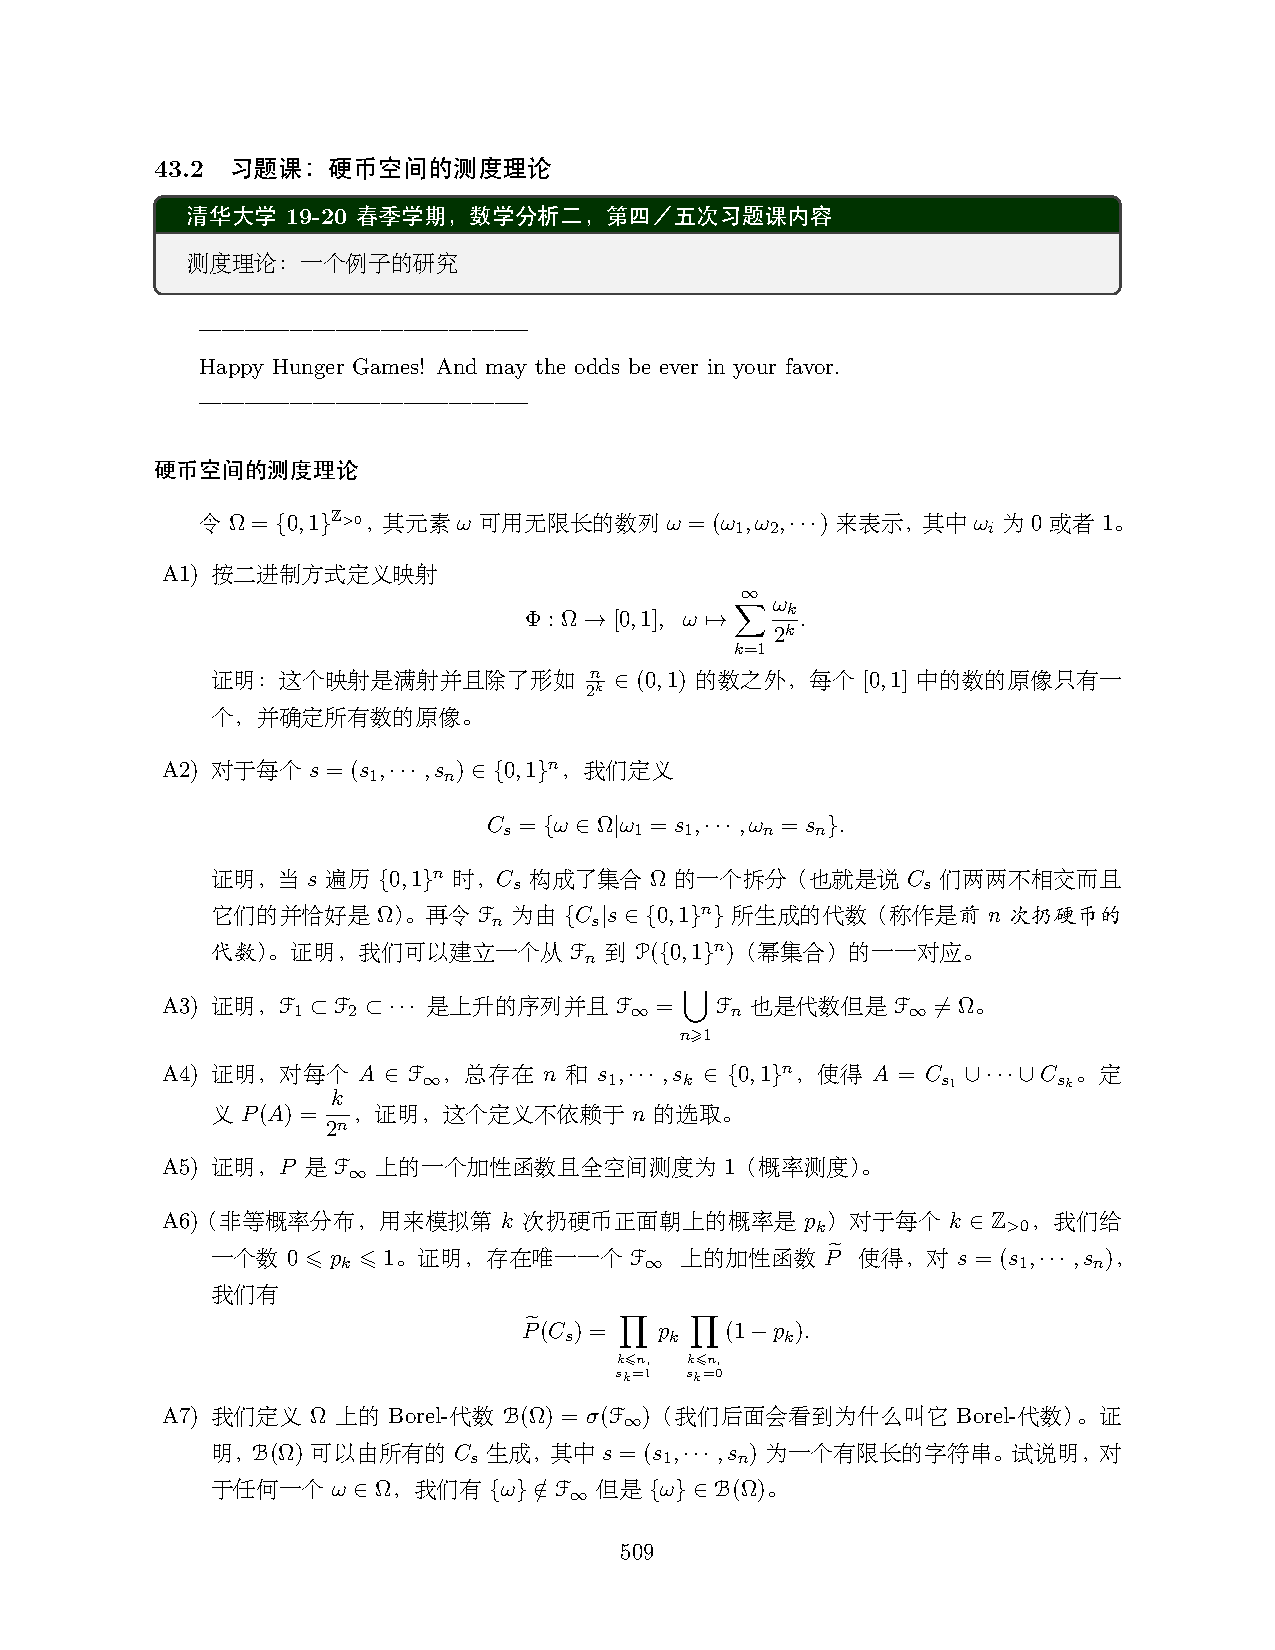
\includepdf[pages=-,pagecommand={\thispagestyle{empty}},scale=.94]{original.pdf}}

\begin{document}
\sourceintro{43.2 习题课：硬币空间的测度理论}{43.2}{509--511}
\section*{所用知识}
第38--40讲的生成元判据、单调类定理和测度扩张。所有独立性均从柱集测度推导；不用强大数定律、遍历定理或零一律。
\section{硬币空间}
令$\Omega=\{0,1\}^{\N_{>0}}$，$\Phi(\omega)=\sum_{k\ge1}\omega_k2^{-k}$，$C_s=\{\omega:\omega_1=s_1,\ldots,\omega_n=s_n\}$，$\mathcal F_n$为长度$n$柱集生成的代数，$\mathcal F_\infty=\bigcup_n\mathcal F_n$，$\mathcal B=\sigma(\mathcal F_\infty)$。
\problem{A1}{证明$\Phi$满射；除$(0,1)$中的二进有理数外每个点原像唯一，并确定全部原像。}
二进制逐位取整算法给出$[0,1)$中每个数的展开，$1$取全一序列。若两序列首异位为$r$，尾项补偿的最大值恰为$2^{-r}$，故只可能为同一前缀后接$1000\ldots$与$0111\ldots$。因此内部二进有理数恰有这两个原像，$0,1$分别只有全零、全一原像，其余唯一。
\problem{A2}{证明长度$n$的$C_s$构成$\Omega$的分划，且$\mathcal F_n$与$\mathcal P(\{0,1\}^n)$一一对应。}
每个序列有唯一的$n$位前缀，故分划。对应将前缀集合$E$送到$\bigcup_{s\in E}C_s$，反向由所包含的分划原子确定。
\problem{A3}{证明$\mathcal F_n$递增，$\mathcal F_\infty$是代数；原文另写$\mathcal F_\infty\ne\Omega$。}
$C_s=C_{s0}\sqcup C_{s1}$给出包含关系。有限多个成员都属于某个共同$\mathcal F_n$，所以对补和有限并封闭。
\fix{$\mathcal F_\infty$是集合族而$\Omega$是样本空间，原比较类型不符。正确的相关结论为$\mathcal F_\infty\ne\mathcal B$，也不等于$\mathcal P(\Omega)$：单点集不属于它，而属于$\mathcal B$，见A7。}
\problem{A4}{证明任意$A\in\mathcal F_\infty$可写成同长度$n$的$k$个不同柱集之并，且$P(A)=k/2^n$不依赖$n$。}
存在$n$使$A\in\mathcal F_n$。将每个长度$n$柱集加细至长度$m\ge n$，恰分成$2^{m-n}$个柱集，所以比值不变。任意两种表示加细到共同长度即可比较。
\problem{A5}{证明$P$在$\mathcal F_\infty$上有限可加，且$P(\Omega)=1$。}
不交集合取公共柱集长度，计数相加即可；全集恰有$2^n$个原子。
\problem{A6}{给定$0\le p_k\le1$，证明存在唯一有限可加函数$\widetilde P$满足
\[\widetilde P(C_s)=\prod_{k\le n:s_k=1}p_k\prod_{k\le n:s_k=0}(1-p_k).\]}
对柱集并定义权重之和。将一个柱集细分为接$0$和接$1$两者，其权重和等于原权重乘$(1-p_{n+1})+p_{n+1}=1$，故定义相容。有限可加性及唯一性由共同加细得到。
\problem{A7}{证明$\mathcal B$由所有有限柱集生成；任意$\omega$满足$\{\omega\}\notin\mathcal F_\infty$但$\{\omega\}\in\mathcal B$。}
各$\mathcal F_n$由柱集有限并组成，所以生成代数相同。$\{\omega\}=\bigcap_nC_{(\omega_1,\ldots,\omega_n)}$可测；任何包含$\omega$的$\mathcal F_n$集合都包含其整个柱集，不能是单点。
\problem{A8}{若$M_j\in\mathcal F_\infty$递减且交集为空，证明某个$M_j$为空。}
否则取$\omega^{(j)}\in M_j$。用逐位抽子列的对角法得到一个序列$\omega$，其前任意有限位在该子列中最终固定。固定$p$，$M_p$只依赖有限位，且从第$p$项以后所取点都在$M_p$，故极限$\omega\in M_p$。于是属于全部$M_p$，矛盾。
\problem{A9}{证明存在唯一$\mathcal B$上的概率测度$P$满足$P(C_s)=2^{-n}$。}
有限可加概率在空交递减列上由A8连续到零，因而为预测度：若不交$A_j$之并$A$仍在代数内，余项$A\setminus\bigcup_{j\le N}A_j\downarrow\varnothing$，其质量趋零，得到可列可加性。扩张定理与有限性给出存在唯一性。
\problem{A10}{证明$\Phi:(\Omega,\mathcal B)\to([0,1],\mathcal B([0,1]))$可测，且$\Phi_*P$为Lebesgue测度。}
各坐标可测，部分和可测，极限$\Phi$可测。二进半开区间$[j2^{-n},(j+1)2^{-n})$的原像与对应柱集仅相差至多两个单点；单点质量由下降柱集为$\lim_m2^{-m}=0$。因此像测度在这些区间上取长度值，利用生成元与概率测度唯一性得到结论。
\problem{A11}{定义$\Psi(x)$为二进制展开，二义时取最终为零者。证明$\Psi$可测且$\Psi_*m=P$（原文末尾还写$=m$）。}
约定$\Psi(1)$为全一序列。每个柱集的原像与相应二进半开区间至多差端点，因而Borel可测、长度为$2^{-n}$。生成元判据及唯一性证明两项。末尾$P=m$分属不同空间，应删去；通过$\Phi,\Psi$在零测集之外对应才是测度空间同构。
\problem{A12}{证明A6的$\widetilde P$可唯一延拓成$\mathcal B$上的概率测度。}
A8与权重无关，故对$\widetilde P$同样保证空交递减列连续到零，重复A9的预测度与扩张论证即可，包括$p_k=0$或$1$的退化情形。
\problem{A13}{令$A_m=\{\omega:\omega_k=1\ (k\ge m)\}$；$B$为含无穷多个零的序列；$C$为零与一均出现无穷次的序列。证明可测并求公平测度。}
$A_m$为坐标事件的可数交，$P(A_m)\le2^{-N}$对任意连续指定的$N$个尾位成立，故为零。$B=(\bigcup_mA_m)^c$，所以$P(B)=1$。同理最终全零集合零测，去掉两种最终常值的序列得到$P(C)=1$。
\problem{A14}{给定严格递增指标$m_k$和指定值$s_{m_k}$，证明$C(s_{m_1},s_{m_2},\ldots)=\{\omega:\omega_{m_k}=s_{m_k}\}$可测；若有$N$个指标，测度为$2^{-N}$，若无穷多个则为零。}
有限指定事件是有限个足够长柱集的并，计数为$2^{-N}$；无穷指定事件是前$N$个约束的下降交，用从上连续性。原题“单调上升”需理解为严格递增，否则重复指标不应重复计数。
\problem{A15}{两组指定指标互不相交，证明相应指定事件$C,D$独立：$P(C\cap D)=P(C)P(D)$。}
有限时联合约束数相加，$2^{-(N+M)}=2^{-N}2^{-M}$。若至少一组无限，则该事件与交事件均零测，等式仍成立。
\problem{A16}{两组有限指定分别有$N,N'$个指标，共同指标有$\widetilde N$个。证明交事件测度为$2^{-(N+N'-\widetilde N)}$或$0$。}
共同位的指定若冲突，交为空；否则联合恰指定$N+N'-\widetilde N$个不同坐标，套用A14。
\section{移位算子与遍历性}
令$S(\omega)_i=\omega_{i+1}$，$\Omega_k=\{\omega:\omega_k=1\}$，$\mathcal G_n=\sigma(\Omega_k:k\ge n)$。
\problem{B1}{证明$S$为$\mathcal B$可测映射。}
$S^{-1}(C_s)=C_{0s}\sqcup C_{1s}$，由生成元判据。
\problem{B2}{证明$\mathcal G_2=S^{-1}(\mathcal B)$。}
拉回$\sigma$-代数由拉回生成元生成，$S^{-1}\Omega_k=\Omega_{k+1}$，故恰为$\mathcal G_2$。
\problem{B3}{证明$\mathcal G_{n+1}=(S^n)^{-1}(\mathcal B)$。}
同理$(S^n)^{-1}\Omega_k=\Omega_{k+n}$。
\problem{B4}{证明$f:(\Omega,\mathcal G_{n+1})\to[0,\infty]$可测，当且仅当$f$为Borel可测且不依赖前$n$位。}
每个$\mathcal G_{n+1}$集合在前$n$位任意改变时不变；用$f$的有理阈值集，得到$f$也不变。反之令$T_{0^n}$为前接$n$个零的映射，它可测，并定义$h=f\circ T_{0^n}$。不依赖前$n$位给出$f=h\circ S^n$，B3使其$\mathcal G_{n+1}$可测。
\problem{B5}{证明$f(\omega)=\limsup_N(\omega_1+\cdots+\omega_N)/N$对尾$\sigma$-代数$\mathcal G_\infty=\bigcap_n\mathcal G_n$可测。}
极限上确界可测；改变有限个坐标只使均值改变$O(1/N)$，不改变$f$。由B4，$f$对每个$\mathcal G_n$可测，所以各Borel原像属于其交。
\problem{B6}{对$\alpha\in[0,1]$，令$X_\alpha=\{\omega:\lim_NN^{-1}\sum_{k\le N}\omega_k=\alpha\}$。证明其不可数，且属于$\mathcal B\setminus\mathcal F_\infty$。}
取基准序列$u_k=\lfloor k\alpha\rfloor-\lfloor(k-1)\alpha\rfloor$，其均值趋于$\alpha$。在平方数位置任意写入一个二进制序列，前$N$位改动不超过$\sqrt N$，均值极限不变，给出不可数多个不同序列。可测性由极限的可数交并表达式。若$X_\alpha\in\mathcal F_n$，非空则包含某个完整$n$位柱集，但这个柱集的尾部可全零或全一，不可能均有同一个频率$\alpha$，矛盾。
\problem{B7}{令$T_s(\omega)=(s_1,\ldots,s_n,\omega_1,\ldots)$。证明对$B\in\mathcal B$，$T_s(B)\in\mathcal B$且$P(T_sB)=2^{-n}P(B)$。}
$T_s(B)=C_s\cap(S^n)^{-1}B$可测。$Q(B)=2^nP(T_sB)$是概率测度，且$Q(C_t)=2^{-|t|}=P(C_t)$，由唯一性$Q=P$。
\problem{B8}{若$S^{-1}A=A$，证明$P(A\cap C_s)=2^{-n}P(A)$。}
迭代得到$(S^n)^{-1}A=A$，故$A\cap C_s=T_s(A)$，应用B7。
\problem{B9}{若$S^{-1}A=A$，证明$\widetilde{\mathcal B}=\{B\in\mathcal B:P(A\cap B)=P(A)P(B)\}$是$\sigma$-代数。}
应谨慎：对一般固定事件$A$，“与$A$独立的所有事件”未必是$\sigma$-代数。这里先由B8及有限可加性知$\mathcal F_\infty\subset\widetilde{\mathcal B}$。概率测度的上下连续性说明$\widetilde{\mathcal B}$是单调类。由单调类定理，它包含$\sigma(\mathcal F_\infty)=\mathcal B$。因此它恰等于$\mathcal B$，当然是$\sigma$-代数。
\problem{B10}{证明移位的遍历性：$S^{-1}A=A$时$P(A)=0$或$1$。}
在B9的等式中取$B=A$，得$P(A)=P(A)^2$，解得结论。
\originalpages
\end{document}
